\chapter{Conclusions}
\label{chap:Conclusions}

%Summary: summarize work and impact, describe directions for further work, describe how this provides a framework for an end to end solution in radio astronomy as well as other domain specific applications
%Goal: show everything worked and was awesome
%State: needs results, should be quick to write but difficult to write now

%TODO: explain this in text
\begin{figure}[ht!]
  \centering
    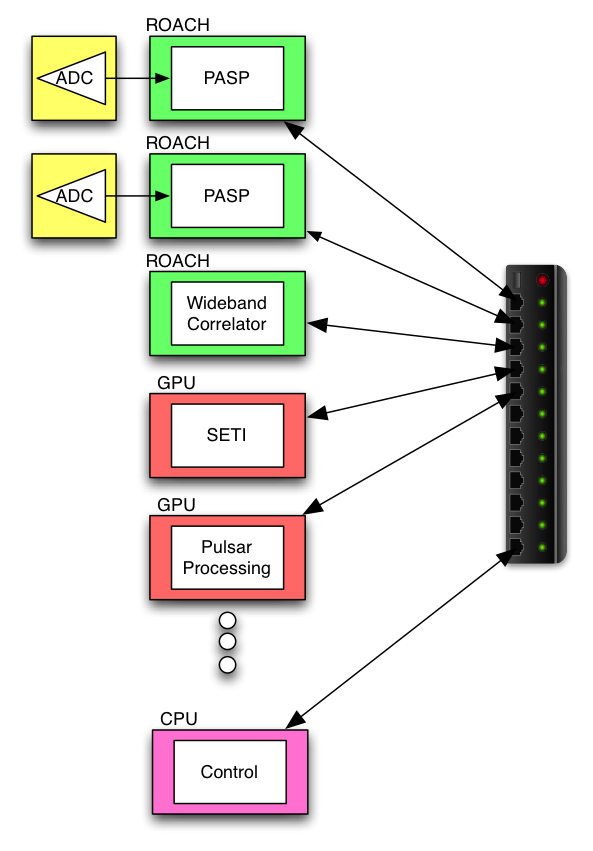
\includegraphics[width=0.5\textwidth]{Images/C5/universal_arch.png}
  \caption{A potential architecture for multiple scientific instruments simultaneously processing data from the same telescope}
  \label{fig: C5/universal_arch.png}
\end{figure}

\section{Future Work}
%Allow blocks to span multiple boards

%Divide blocks between boards (?)

%Design algorithm aspects like 

%Do a better job of preserving symmetry

%Use for other fields

%Design interconenct